\section{衰老与秀丽隐杆线虫}

衰老是生命活动中一种极为复杂的生物学现象,它贯穿生命的整个历程。从分子层面 的微观变化,到器官乃至整个系统的宏观转变,无一不彰显着这一过程的深远影响。在生 物体衰老的过程中,细胞功能会逐渐衰退,细胞的代谢活性也随之降低。与此同时, 氧化应 激会不断在体内积累\upcite{lopez-otin_hallmarks_2023}。此外, DNA 修复能力也会逐渐丧失, 这些变化相互交织、相互影 响,最终使得生物个体的生存能力逐渐降低、适应能力下降、生命走向衰退\upcite{noauthor__nodate-1}。近年来, 衰 老研究逐渐成为生物医学领域的热点,不仅因为衰老是许多慢性疾病的主要风险因素,而 且它是人类健康寿命延长的重要方向\upcite{olshansky_implausibility_2024}。为了深入探索衰老的分子机制,科学家们开发了 多种模型生物,其中秀丽隐杆线虫因其独特的优势成为研究衰老的重要工具\upcite{jeayeng_caenorhabditis_2024} (图\ref{fig:worm_aging})。

\begin{figure}[H]
    \centering
    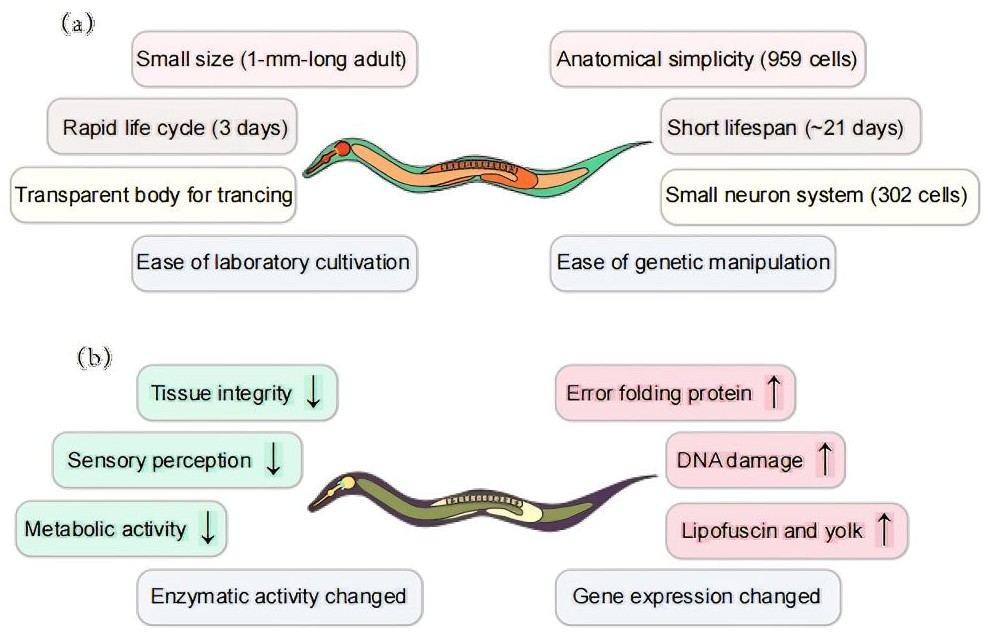
\includegraphics[width=0.8\textwidth]{img/worm_aging.jpg}
    \caption{线虫结构以及线虫衰老过程中的生理变化:(a) 线虫基本的身体数据;(b) 线虫在衰老过程中的生理变化}
    \label{fig:worm_aging}
\end{figure}

秀丽隐杆线虫因其生命周期短、遗传背景简单、易于操作以及完全测序的基因组等特 点,已成为研究衰老和发育生物学的理想模型生物\upcite{jeayeng_caenorhabditis_2024}。在秀丽隐杆线虫的衰老研究中,成 虫期从其被孵化后的第 1 天开始算起,其生殖期通常处于第 3-4 天,而衰老的迹象则从线 虫的第 8 天左右开始显现\upcite{jeayeng_caenorhabditis_2024}(图\ref{fig:worm_aging})。因此在研究中, 第一天被视为线虫成虫期的起点, 第 八天被视为线虫发生明显的衰老的时间线。这种时间上的对应关系使得科学家能够通过对 线虫进行不同时间点的比较,研究衰老的动态过程。

\section{胞间连接及组织屏障}

胞间连接是细胞间进行通信和物质交换的重要途径。细胞间的三种连接方式为紧密连 接,粘附连接和间隙连接。其中,紧密连接发挥着渗透屏障作用,粘附连接负责固定、维 持组织中细胞间的相对位置,间隙连接则负责信号传递(图\ref{fig:cell_connection})。

\begin{figure}[H]
    \centering
    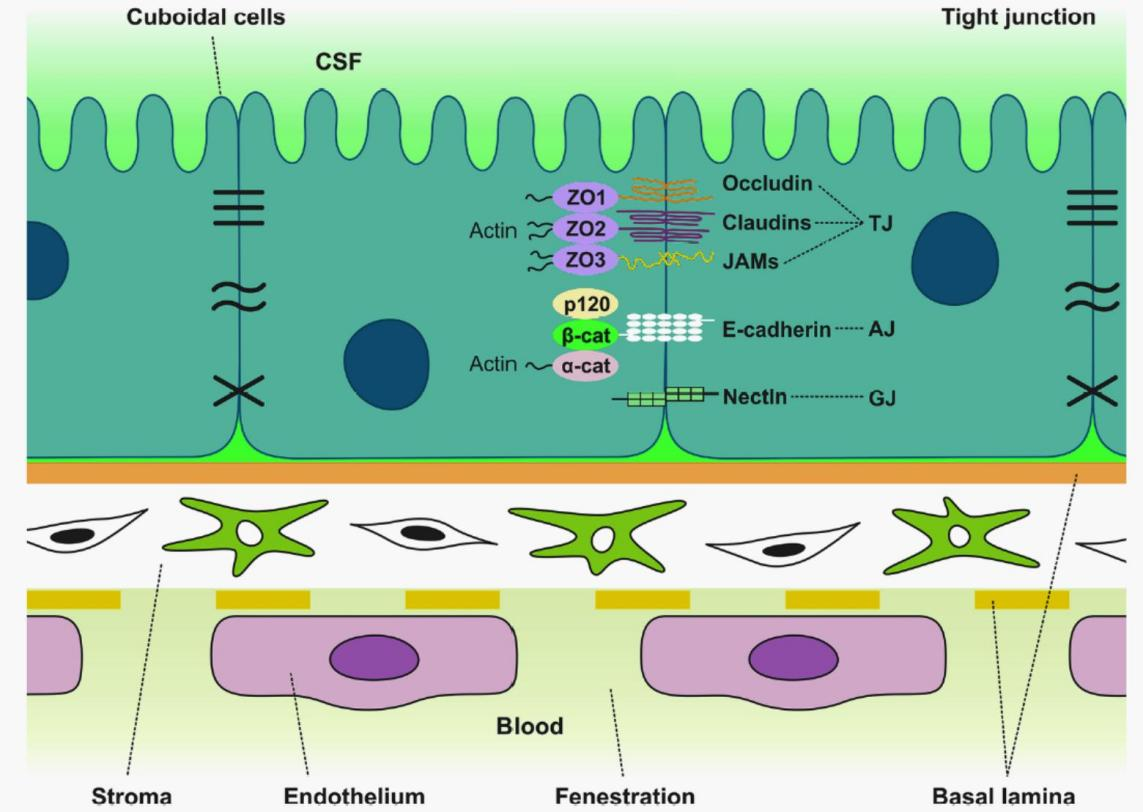
\includegraphics[width=0.8\textwidth]{img/three_cell_link_functions.jpg}
    \caption{细胞间连接的三种方式:紧密连接、粘附连接和间隙连接}
    \label{fig:cell_connection}
\end{figure}

在线虫中,胞间连接主要通过缝隙连接实现。缝隙连接是一种特殊的细胞间结构,允 许小分子在相邻细胞之间直接传递。这种连接在多种生理过程中起着关键作用,包括发育 调控、代谢协调和应激响应等\upcite{wang_structural_2024}。在线虫中, HMR-1 蛋白是一种重要的缝隙连接蛋白, 且 HMR-1 与哺乳动物的连接蛋白具有高度同源性。HMR-1 在线虫的多种组织中表达,包括 表皮、肠道和生殖器官等(图\ref{fig:HMR-1_protein})。研究表明, HMR-1 不仅参与了细胞间的直接通信, 还 在胚胎发育、组织屏障功能和环境应激反应中发挥重要作用\upcite{naturale_persistent_2023}。

\begin{figure}[H]
    \centering
    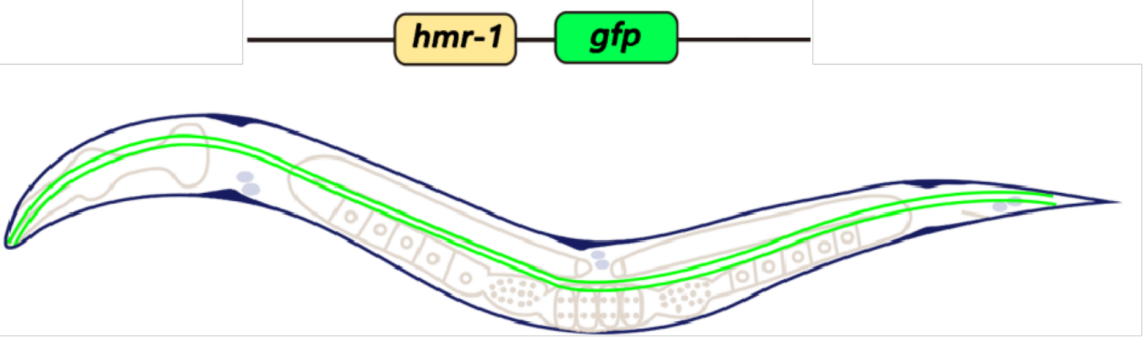
\includegraphics[width=0.8\textwidth]{img/HMR_worm.png}
    \caption{实验用绿色荧光蛋白标记 HMR-1 来显示线虫的表皮屏障示意图}
    \label{fig:HMR-1_protein}
\end{figure}

线虫的组织屏障主要包括表皮屏障和肠道屏障,这两种屏障在维持线虫的内环境稳定  和防御外界病原体侵害中起着关键作用(图\ref{fig:worm_barrier})。线虫的表皮屏障由外层的表皮细胞构成,

主要负责保护线虫免受外界机械损伤和病原体的侵害。表皮细胞通过紧密连接形成了一种 屏障结构,防止有害物质从外界进入线虫体内\upcite{zhang_structural_2015}。肠道屏障是线虫消化系统的重要组成部 分,主要由肠道上皮细胞构成。肠道屏障的主要功能是吸收食物中的营养物质, 同时防止 有害物质扩散进入线虫体内。线虫肠道上皮细胞通过紧密连接,发挥选择性通透性屏障的 作用,确保营养物质的吸收和有害物质的排除\upcite{tan_killing_1999}。

\begin{figure}[H]
    \centering
    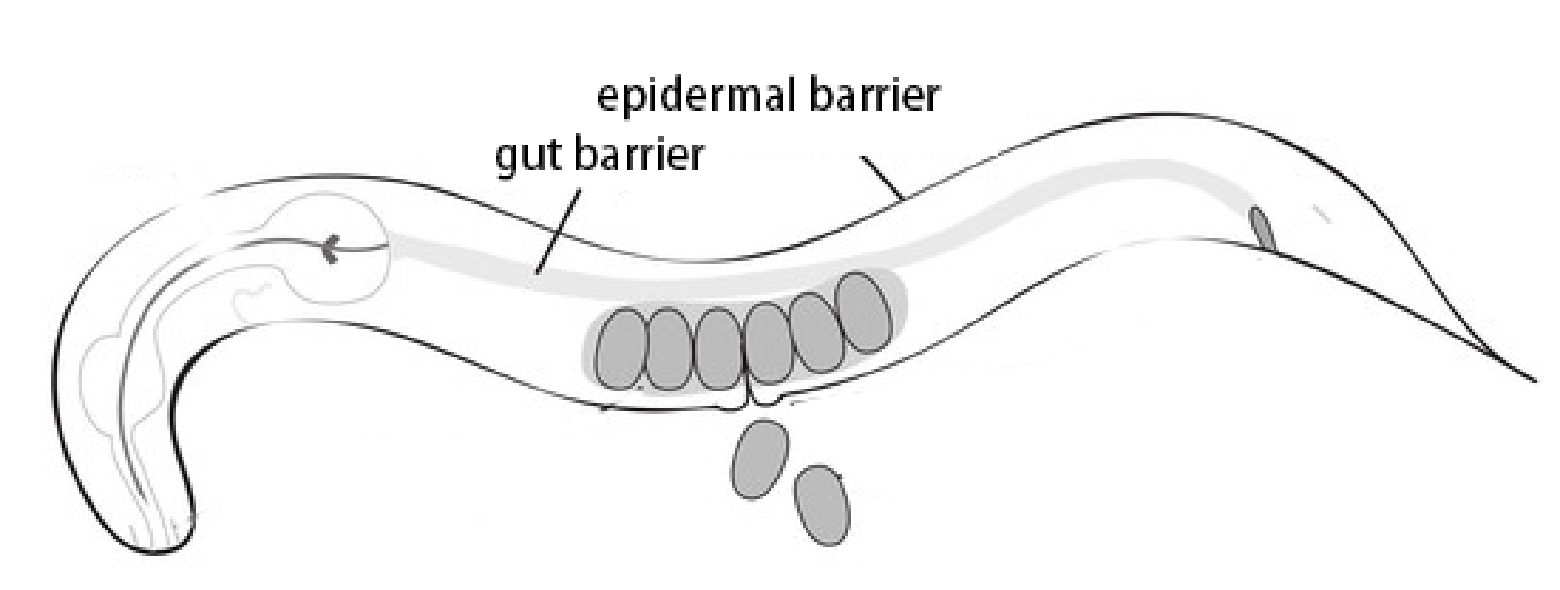
\includegraphics[width=0.8\textwidth]{img/worm_blocks.png}
    \caption{线虫的组织屏障示意图}
    \label{fig:worm_barrier}
\end{figure}

胞间连接和组织屏障在功能上具有密切的联系。胞间连接的异常状态会导致组织屏障 的功能发生障碍, 进而影响线虫的整体生理状态\upcite{wang_structural_2024}。因此, 通过对线虫 HMR-1 蛋白和组织 屏障的研究,可以为开发新的临床治疗策略提供理论依据。

\section{组织蛋白酶}

\begin{figure}[H]
    \centering
    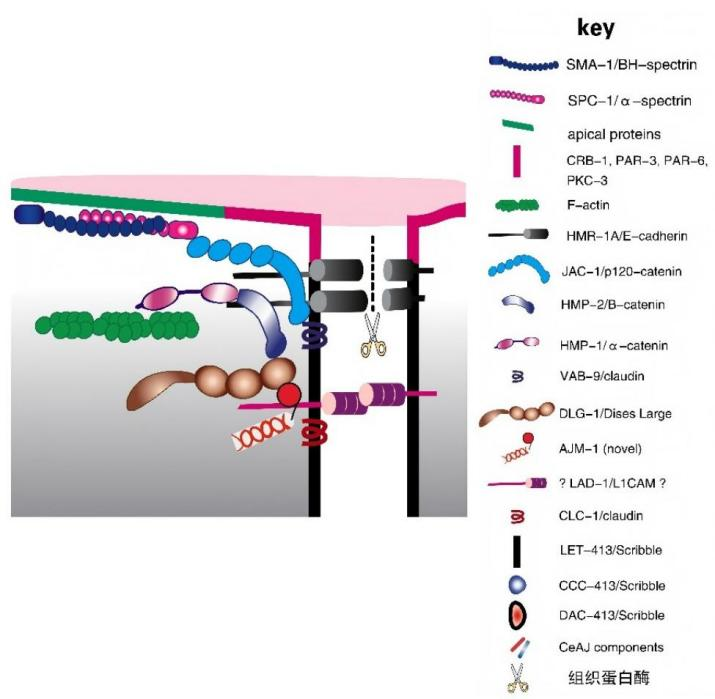
\includegraphics[width=0.5\textwidth]{img/protease.jpg}
    \caption{组织蛋白酶破坏细胞间连接示意图}
    \label{fig:protease}
\end{figure}

组织蛋白酶是一类能够特异性分解细胞外基质成分的蛋白酶,广泛参与组织修复、细胞迁移、胚胎发育和疾病发生\upcite{jakos_cysteine_2019} 等过程\upcite{wang_cathepsins_2023}。在线虫中, 组织蛋白酶在细胞屏障的维持、胞 间连接的调控以及生理和病理过程中都具有重要的功能\upcite{teuscher_longevity_2024}。组织蛋白酶可能会通过调节细 胞外基质的成分,间接影响胞间连接的结构和功能。然而,组织蛋白酶的过度表达可能导 致细胞连接的稳定性失调,破坏细胞间的通信以及组织屏障(图\ref{fig:protease})。

\section{研究不同种类之间同源物的意义}

在生物学种系发生理论中,若两个或多个结构具有相同的祖先,则称它们同源。这里 相同的祖先既可以指演化意义上的祖先, 即两个结构由一个共同的祖先演化而来, 比如,蝙 蝠的翅膀与人类的手臂是同源的;也可以指发育意义上的祖先, 即两个结构由胚胎时期的 同一组织发育而来,例如,人类女性的卵巢与男性的睾丸同源。总而言之,若两个或多个 基因、蛋白、结构、组织或器官等具有相同的祖先,则称它们互为同源物。

在生物学研究中, 同源物的研究具有多方面的重要意义。比如,科学家可以通过比较 同源基因或者蛋白质,确定物种之间的亲缘关系,构建进化树,预测基因功能以及进行基 因注释等。而通过研究不同物种之间的同源物,尤其是人类在不同模式生物中的同源物对 于开发针对人类不同疾病的治疗方法等极为关键。这种方法不仅高效有用,而且能够最大 程度上降低生物实验的成本,对于科研人员具有重要的科研价值和实际应用意义。

\section{RNAi实验在线虫中的应用}

RNAi干扰是一种分子生物学上由双链RNA诱发的基因沉默现象,其机制是通过阻碍  特定基因的转录或翻译来抑制基因表达。当细胞中导入与内源性mRNA编码区同源的双链 RNA时,该mRNA会发生降解从而导致基因表达沉默\upcite{mello_revealing_2004}。
	
在线虫中,RNAi 实验应用广泛\upcite{tabara_rde-1_1999}。它不但能够研究基因的功能,还能够确定信号通路 中不同基因的上下游关系,帮助我们理解细胞里的信息传递网络。线虫对 RNAi 反应敏感 高效,只需要通过喂食,就能轻松把 dsRNA送入线虫体内,引发 RNAi 反应。RNAi 实验在 线虫中的意义重大。它不仅推动了研究人员对线虫基因功能的认识,还为理解人类基因功 能和疾病机制提供了线索。而在我们的实验中之所以选择 RNAi 来敲低目的基因,是因为 我们的实验需要筛选目的基因,该试验便于进行大规模的基因筛选。

\section{小结}

本章节从衰老这一生命活动的复杂生物学现象出发, 阐述了秀丽隐杆线虫作为研究衰 老的重要模式生物的优势;进而深入探讨了胞间连接里紧密连接、粘附连接和间隙连接的 功能,且着重介绍了线虫缝隙连接及 HMR-1 蛋白的关键作用;接着又介绍了线虫组织屏障的构成与功能,以及胞间连接与组织屏障的密切联系;随后聚焦于组织蛋白酶, 阐述其 广泛参与多种生理病理过程的现象及其对胞间连接和组织屏障的潜在影响;最后介绍RNAi 实验原理及在线虫中的应用优势, 为后续基于 RNAi 的基因功能研究实验介绍奠定了 基础。
